\documentclass[11pt]{article}
\usepackage[T1]{fontenc}
\usepackage[utf8]{inputenc}
\usepackage[margin=1in]{geometry}
\usepackage{amsmath,amssymb,booktabs,graphicx,hyperref,array}
\setlength{\emergencystretch}{2em}
\hypersetup{colorlinks=true,linkcolor=blue,citecolor=blue,urlcolor=blue}
\title{When Oracle Low-Rank Error Repair Helps or Harms\\Intervention Predictions}
\author{Author information to be supplied}
\date{November 4, 2026 --- private working manuscript, version 15}
\begin{document}
\maketitle
\begin{abstract}
A response space fitted from native vector changes without readout labels concentrates a highly repairable component of intervention-prediction error. In a fresh Qwen-0.6B layer-21 test, oracle repair in the historical rank-eight space reduces is/are readout MSE by 99.25\%. On separate fresh contexts, prior-centered ridge correction reduces the historical predictor's MSE by 97.21\%. Strong direct predictors and subsequent small-budget fits show that this learned usefulness has unstable comparative advantage. Rank controls, other frames and other checkpoints delimit the result: larger spaces can improve further, and oracle repair can also harm. The contribution is a controlled empirical chain from vector-fitted response structure through oracle repairability to learned usefulness, its resource costs and its transfer limits.
\end{abstract}

\section{Introduction}
A model of an internal intervention is useful when its predicted vector change produces the right downstream effect. This study asks whether a response space selected from native vector data identifies a correctable component of prediction error, and whether that component can be learned well enough to help on new contexts. We follow the same prediction through vector error, oracle repair, learned correction, direct baselines and transfer.

The starting point is historical E041: on Qwen3-0.6B-Base, correcting error inside a rank-eight response space reduced the is/are readout MSE by 98.85\%, compared with 14.44\% outside. The original forecast favored outside repair; this favorable layer-21 regime was therefore selected historically. Three subsequent 64-block TEST cohorts separate replication of that observation, learned correction and label-budget comparisons. A later three-fit/readout study probes the stability of the small-budget result on a reused cohort (Table~\ref{tab:scope}).

The central finding survives the move from diagnosis to prediction, with a clear change in interpretation. A space chosen without direct readout labels supports almost complete oracle correction on fresh lexical pairs. A learned prior-centered correction substantially improves the historical predictor on another fresh cohort. Full-vector direct ridge has lower mean loss at the matched additional training budget. A correction advantage at 32 labels appears in one fixed training sequence, while three later FIT32 draws give mixed rankings. Separate layer/frame tests include both benefit and harm. Together these results establish a useful empirical structure whose predictive and comparative value depends on the fitting and evaluation regime.

\begin{table}[ht]\centering\scriptsize
\setlength{\tabcolsep}{4pt}
\begin{tabular}{>{\raggedright\arraybackslash}p{.19\textwidth}>{\raggedright\arraybackslash}p{.36\textwidth}>{\raggedright\arraybackslash}p{.36\textwidth}}\toprule
Study & Data and reuse & Inference and role\\\midrule
L21 oracle/rank & First 64-block TEST; historical B5/$U$; rank controls use three disjoint eight-block FIT groups & Frozen operators and forecasts; nominal paired block intervals conditional on fixed fits.\\[3pt]
L21 learned384 & Second 64-block TEST; reuses all 24 FIT blocks, 384 vector labels & Prospective readout test; primary C-minus-P and secondary C-minus-Direct contrasts.\\[3pt]
L21 budget & Third 64-block TEST; one fixed FIT0/seed17 sequence at 32--256 labels, full pool at 384 & Prospective fixed-fit TEST; primary C32-minus-Direct32 contrast.\\[3pt]
Three FIT32/readout & Six new FIT blocks, three disjoint two-block fits; reuses budget TEST posthoc; adds have/has & Conditional nominal intervals; mixed per-fit rankings; readout transfer on the same contexts.\\[3pt]
Aligned and earlier tests & Qwen L27/Gemma-270M L17 share 256 lexical blocks; earlier Gemma-1B/Llama cohorts are separate & Three fixed fits/aligned model; nominal T5 intervals. Earlier single-fit families retain their original corrections.\\[3pt]
Forecast/diagnosis & Aligned Qwen; supporting 32-block scopes; historical/current Gemma fitted-object crosses & Descriptive sign/utility summaries and posthoc matrix substitutions.\\\bottomrule
\end{tabular}
\caption{Scope of the evidence. The three L21 TEST cohorts are distinct; the later FIT32 study reuses the third. Conditions, fits and shared cohorts retain their dependence. The supplement gives complete protocols, chronology and result tables.}\label{tab:scope}
\end{table}

\section{Relation to existing work}
Engels et al.~\cite{engels2024} decompose and partially repair sparse-autoencoder reconstruction error, measuring downstream cross-entropy. Here the target is a native intervention delta and the outcome is squared error in its predicted grammatical logit-margin effect. The empirical extension is the linked sequence of response-space fitting, fresh oracle replication, rank/norm controls, learned correction and resource-aware baseline comparison.

Subspace activation patching, self-repair and computational-graph methods provide established context~\cite{makelov2023,rushing2024,ameisen2025,farnik2025}. Deshpande~\cite{deshpande2026} studies preservation of refitted ridge readouts under sparse compression; our spaces instead derive from native vector responses and are tested by finite interventions through the native suffix. Guo et al.~\cite{guo2026} establish gradient-based intervention attribution and feature selection, directly preceding the gradient forecasting used here. Luo et al.~\cite{luo2026} show why intervention comparisons need strength, surface and basis matching. Our random-space and norm controls address specified parts of that comparison. Prior-centered ridge and kernel mean functions are standard regression constructions~\cite{rasmussen2006}. The contribution rests on the measurements and their controlled comparisons.

\section{Prediction, correction and experimental design}
\subsection{Native response and oracle diagnostic}
For intervention $I$, let $D=y_I-y_0$ be the native target-branch output change. A target-free input representation predicts $P$. An orthonormal $U\in\mathbb R^{d\times r}$ is fitted from native vector responses; the historical space has $r=8$. Let $g_I(v)$ be the actual native-suffix logit margin after inserting $y_0+v$, holding the intervention's upstream residual fixed. With the same reference margin for target and prediction, squared error is
\[
 L(v)=[g_I(D)-g_I(v)]^2.
\]
The oracle diagnostics insert
\[
 P_U=P+UU^\top(D-P),\qquad P_{out}=D-UU^\top(D-P).
\]
Both access true TEST $D$. Inside repair removes the vector-error projection onto $U$, and outside removes its complement. Their downstream effects are measured through the suffix. If $e=g_I(D)-g_I(P)$ and $a=g_I(P_U)-g_I(P)$, the loss change is $a^2-2ea$. Positive change denotes worse prediction of the intervention effect.

The L21 experiments use Qwen3-0.6B-Base and the literal E041 upstream intervention. At the final prompt position, layer-19 SwiGLU coordinate 1317 moves toward its donor value at dose .5 or 1. Branch B leaves layer 20 free; branch C restores recipient coordinate 1423. Each lexical block has four subject/attractor-number forms and 16 branch/dose conditions. Donors reverse subject number in the F1 prompt, ``The \{subject\} that the \{attractor\} can see''. The target is layer-21 output; the exact native L22--27 suffix supplies the is/are readout. Native arithmetic is FP32, fitting/projection FP64, with separately qualified suffix batching. B5 uses a native ridge predictor.

The frozen input is $x=[\Delta x_{20}/s_{20},\Delta x_{21}/s_{21}]/\sqrt2$, and historical $P=\operatorname{FP32}(xWU^\top)$. These features require native upstream prefixes while avoiding the layer-21 output being predicted. TEST forecasts are globally frozen before the new native targets. The three new rank-study predictors use eight FIT blocks each (128 labels), fixed ridge penalty $10^{-4}$, six nested SVD ranks and fixed Gaussian-QR random spaces. A separate random arm rescales its correction to the FIT-space correction norm.

\subsection{C is ridge around a historical prior}
The learned correction fits coefficients of $(D-P)U$ and predicts $C=P+f_C(x)U^\top$. Same-$U$ fits $DU$; Direct fits full $D$. The shared estimator centers inputs and targets, uses $K+n\lambda I$, and adds the training target mean. Linear and RBF kernels use the grid $\lambda\in\{1,10^{-2},10^{-4},10^{-6}\}$; the RBF scale is the median positive training squared distance. Vector-only block CV selects models.

In exact arithmetic with $P=xWU^\top$, centered design $A=X-\bar X$ and $Y=DU$, the linear C fit is
\[
 \Gamma_C=\arg\min_\Gamma\big\{\|Y_c-A\Gamma\|_F^2+n\lambda\|\Gamma-W\|_F^2\big\},
 \qquad \widehat Y_C(x)=\bar Y+(x-\bar X)\Gamma_C.
\]
This is ridge centered on $W$, with an unpenalized intercept; same-$U$ shrinks toward zero. The implementation's FP32 P introduces a rounding qualification. RBF C is residual kernel ridge around mean function $xW+\overline{Y-XW}$. The supplement gives the exact smoother identities and implementation audit, including the conditions under which projected Direct equals same-$U$.

C and Direct search eight linear/RBF candidates in the learned384 and original budget studies; same-$U$ searches the four linear candidates. In the later three-FIT32 study, every method searches all eight. At 384 labels, all methods choose linear/$10^{-6}$, the grid's lower boundary. The original 32-label models all choose linear/$10^{-4}$. Two-block CV at 32 labels trains on one block per fold.

Historical information is a real resource. C inherits $W,U$ and scales; same-$U$ inherits $U$ and scales. E036's prior-development pool had 512 target rows across 128 documents with fitting and selection roles. Its ledger records 640 network, 640 CLT, 512 JVP and 512 target operations, beyond the subsequent vector-label budget. The supplement retains the full cost and selection chronology.

\subsection{Sampling, inference and companion data}
The independent sampling unit is the lexical block. The L21 analyses average 16 conditions within each of 64 blocks; aligned studies average fits and conditions within each of 256 blocks. Reported nominal 95\% intervals use the saved 1,999-draw paired block bootstrap and condition on fixed fitted objects. Original Gemma/Llama families retain their distinct saved correction rules. Every stage has its own independent scientific completion receipt; the manuscript uses saved analyses without refitting or resampling.

The companion transcoder study shares Qwen L27 states and 4,096 unit-dose native/first-fit ridge margins. Its ridge uses 128 FIT\_MAP labels; Direct256 here uses a different pooled training budget. The L21 cohorts and Gemma agreement tests have separate native acquisitions. Full reuse mappings and model identities are in the supplement.

\section{L21 results: repairability, usefulness and comparison}
\subsection{A vector-fitted space concentrates oracle benefit}
On the first fresh 64-block TEST, inside repair reduces historical B5 MSE by 99.25\%, compared with 8.38\% outside (Table~\ref{tab:oracle}). The inside-minus-B5 contrast is $-.0144172$, nominal 95\% interval $[-.0160698,-.0129072]$. Reductions range from 99.07\% to 99.30\% across the four branch/dose marginal groups. The historical rank-eight vector-fitted space therefore identifies a sharply repairable component on new lexical pairs.

\begin{table}[ht]\centering\small
\begin{tabular}{lrr}\toprule Historical fit/repair & Readout MSE & Reduction from B5\\\midrule
B5 prediction & .01452685 & ---\\
Oracle inside, rank 8 & .00010961 & 99.245\%\\
Oracle outside & .01330943 & 8.381\%\\
Full oracle & $1.31\times10^{-11}$ & Numerical floor\\\bottomrule\end{tabular}
\caption{First L21 TEST: 64 fresh blocks, 1,024 conditions, frozen historical fit. Oracle arms use true TEST error. Inside and outside have unequal rank/norm budgets; the full-oracle residual is the FP32 patch/suffix floor.}\label{tab:oracle}
\end{table}

The separate three-fit rank study supplies controlled alternatives on the same TEST. Baseline MSE is .00075285. At rank eight, FIT-space repair gives .00008939, an 88.13\% reduction, versus 1.18\% for fixed equal-rank random spaces and 5.30\% for norm-rescaled random corrections. The saved FIT-space paired contrast is $-.00066347$, interval $[-.00081751,-.00052898]$. Figure~\ref{fig:ranks} retains all six ranks: the reductions rise to 94.14\% and 96.90\% at ranks 16 and 32. These controls support response-derived structure while also showing scope for larger spaces.

\begin{figure}[ht]\centering
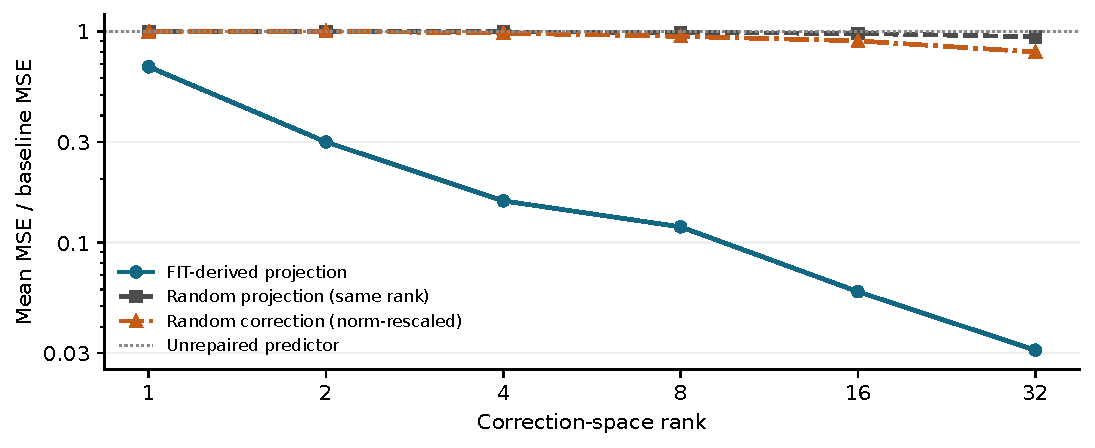
\includegraphics[width=.87\textwidth]{l21_rank_controls.pdf}
\caption{Three fixed new fits on the first 64-block TEST; means normalized by their common baseline. Rank and random seeds were fixed before outcomes. FIT-derived and random projections share rank; the rescaled arm matches correction magnitude. Points summarize these fixed controls.}\label{fig:ranks}
\end{figure}

\subsection{Learned correction is useful against P; Direct384 has lower mean loss}
On a second fresh 64-block TEST, C trained on the existing 384 FIT vector labels reduces P's readout MSE by 97.21\% (Table~\ref{tab:learned}). Its primary C-minus-P contrast is $-.0149633$, nominal interval $[-.01669,-.01329]$. This is downstream improvement with forecasts frozen before true TEST error becomes available.

\begin{table}[ht]\centering\small
\begin{tabular}{lrr}\toprule Arm & Readout MSE & Vector squared error\\\midrule
Historical P & .01539272 & 4.08662\\
Prior-centered C & .00042944 & 2.89175\\
Same-$U$ direct & .00040599 & 2.88978\\
Direct384 & .00032652 & .29801\\
Mean correction & .01605005 & 4.07251\\
Oracle inside & .00008828 & 2.84390\\
Zero-change & .76689144 & 5.93717\\\bottomrule\end{tabular}
\caption{Second L21 TEST: 64 blocks and frozen fits using 384 reused vector labels. Vector error is mean squared L2. Oracle is diagnostic; zero-change predicts the original natural margin. Inference is conditional on fixed fits.}\label{tab:learned}
\end{table}

The secondary C-minus-Direct384 contrast is $+.000102919$, nominal interval $[+.000036397,+.000174289]$. Direct384 has 23.97\% lower mean loss than C; equivalently C has 31.52\% higher loss. Same-$U$ also has slightly lower point loss, while constant FIT-mean correction worsens P. C improves P across every reported branch/dose/subject/attractor marginal group. Direct384 has lower means in both branches and doses; one descriptive subject subgroup slightly favors C. Complete subgroup values remain in the supplement and evidence.

\subsection{A small-budget advantage depends on the fit}
A third fresh 64-block TEST compares one fixed FIT0/seed17 training sequence. Table~\ref{tab:budget} shows every budget. The 384-label models use the full pool, extending the lower-budget sequence with FIT0 blocks. At 32 labels, the primary C-minus-Direct contrast is $-.000809242$, nominal interval $[-.001215298,-.000446333]$: a 48.03\% MSE reduction. With the shared linear/$10^{-4}$ smoother, C versus same-$U$ differs through the historical prior; C versus Direct also changes the output span.

\begin{table}[ht]\centering\small
\begin{tabular}{rrrr}\toprule Vector labels & C & Same-$U$ & Direct\\\midrule
32 & .000875571 & .001435104 & .001684814\\
64 & .001275866 & .000927738 & .000790169\\
128 & .000767452 & .000696753 & .000481287\\
256 & .000489643 & .000496114 & .000440074\\
384 & .000342340 & .000321220 & .000308196\\\bottomrule\end{tabular}
\caption{Third L21 TEST: is/are MSE on 64 blocks, conditional on one fixed training sequence. $P=.015209579$. Direct has lower means at 64--384 labels; the 256/384 C-minus-Direct intervals include zero. The original learned384 study in Table~\ref{tab:learned} uses a different TEST cohort.}\label{tab:budget}
\end{table}

Three subsequent two-block FIT cohorts acquire 32 labels each and reuse this third TEST posthoc. On have/has, mean MSE is .001598713 for C and .001230636 for Direct: C-minus-Direct $+.000368077$, nominal interval $[+.000134272,+.000653699]$. On is/are, the mean contrast is $+.000172888$, interval $[-.000127204,+.000484746]$. Per-fit is/are contrasts are $+.000746091,-.000015488,-.000211940$; have/has contrasts are $+.000369036,+.001108920,-.000373724$. The mixed signs preserve the observed original C32 advantage while limiting its stability across new fits and readouts.

The supplementary implementation audit explains two numerical/semantic details of this follow-up. Saved P vectors and is/are margins are identical to the budget study; its tiny P-MSE difference comes entirely from recomputing the native reference through another numerical path (maximum margin difference $1.90735\times10^{-5}$). The arm named zero inserts zero MLP21 delta while retaining the intervened residual, whereas earlier zero-change uses the original natural margin. All raw records are preserved.

\section{Transfer and policy results bound the interpretation}
The aligned layer-27 Qwen and layer-17 Gemma-270M tests use three fixed matched predictor/space pairs per model and the same 256 lexical blocks. The same three Qwen fitted pairs help on T2 and harm on T5 (Table~\ref{tab:aligned}); Gemma benefits on both frames. Outside-space repair has lower pooled loss in these cells, with a substantially larger dimension/norm budget. Per-fit reversals and full inside/outside tables are retained in the supplement.

\begin{table}[ht]\centering\small
\begin{tabular}{llrrl}\toprule Model & Frame & P MSE & Inside-minus-P & Nominal 95\% interval\\\midrule
Gemma-270M & T5 & .449097 & -.116462 & [-.144036,-.091732]\\
 & T2 & .209279 & -.126023 & [-.140182,-.113846]\\
Qwen-0.6B & T5 & .490827 & +.044905 & [+.013197,+.076805]\\
 & T2 & .672181 & -.139841 & [-.177426,-.107007]\\\bottomrule\end{tabular}
\caption{Aligned 256-block tests, conditional on three fits/model. T5 is primary; T2 is descriptive. Model, layer and fitting recipe differ from the L21 studies.}\label{tab:aligned}
\end{table}

Earlier separate single-fit 256-block tests establish T5 harm in Gemma-1B ($+.50370$, saved 99\% interval $[.43370,.57832]$, adjusted $p=.003$) and Llama-1B ($+.77826$, $[.66913,.89066]$, adjusted $p=.002$). Llama's secondary T2 effect is beneficial, $-.40679$ ($[-.47176,-.35053]$). Gemma's predicted vector/readout ranking reversal fails: the space removing more vector error also has lower fresh T5 readout loss. Posthoc old/new matrix substitutions show that the mean ranking follows the subspace-pair version on both fixed cohorts. The supplement preserves the full crossed table and original family definitions.

The separate L27 learned gate makes the distinction between sign forecasting and useful policy concrete. A local score $(Jc)^2-2(Jr)(Jc)$ uses native readout gradient $J$, residual $r=D-P$ and correction $c=UU^\top r$ to forecast finite loss-change signs. Replacing $r$ by a learned residual gives a deployable-with-prefix/gradient-access gate. On Qwen T5/T2, oracle sign accuracies are 99.479\%/99.837\%; learned accuracies are 64.746\%/68.620\%, versus constant-rule 63.249\%/59.375\%. Yet T5 gate loss .521107 exceeds P's .490827, and Direct256 has lower mean loss on both frames. These accuracies are dependent-cell descriptive fractions.

Supporting 32-block scopes reinforce that limit: learned sign accuracies on Gemma-1B/Llama-1B/Gemma-270M are 39.84\%/65.62\%/58.07\%, below constant-rule 60.94\%/72.40\%/62.50\%. Each learned gate loses to the better always/never policy. Complete loss tables, all matched crosses and timing qualifications are in the supplement.

\section{Limitations and interpretation}
The evidence concerns selected synthetic contexts, native branches and grammatical two-token margins. Fresh lexical pairs test the historically selected L21 regime; they leave model/frame/layer generalization conditional. The have/has extension changes a readout on reused prompts. Differences between L21, aligned and earlier tests also change operators and fitting recipes, so they cannot isolate layer as the cause of different repair signs.

Oracle correction requires true TEST error. Learned C avoids that access, while still requiring native upstream features and historical fitting information. Equal additional label budgets leave those prior resources unequal. Current C-versus-Direct comparisons also change the output span; the full-vector residual comparator would separate that factor, but has no approved result in this article. Kernel grids, fixed random draws and the three later FIT32 cohorts bound the conclusions to the tested choices.

Intervals condition on fitted objects and sample lexical blocks. The newer nominal analyses, older adjusted families and posthoc diagnostics have separate inferential scopes. In particular, two negative per-fit C32 contrasts coexist with a three-fit is/are interval crossing zero, and point rankings at budget256/384 leave the corresponding contrasts uncertain. Scientific completion approvals verify the recorded execution and evidence; external replication remains open.

The resulting thesis is specific and positive: native vector-fitted response structure can concentrate readout-relevant prediction error strongly enough to support fresh oracle repair and useful learned correction. Direct baselines, rank controls and transfer tests define where that usefulness holds. The supplementary report provides the complete historical record, forensic checks and operation receipts. Authorship, public evidence location and release disclosures remain to be completed before submission.

\clearpage
\small
\bibliographystyle{plain}
\bibliography{references}
\end{document}
